\input{../../../plantilla.tex}

\encabezados[Programación Matemática 1]{Hugo García}
\titulos[Práctica 1]{Programación Matemática 1}

\begin{document}
	
	\thispagestyle{encabezado}
	\pagestyle{general}
	\onehalfspacing
	
	\begin{center}
		\Huge{\underline{\textbf{Examen Final}}}
	\end{center}
	
	\section{Problema 1}
	
	Notemos que en cada nuevo cálculo del problema, tenemos que 
	\begin{align*}
		F(1)=0, && F(2)=4, && F(3)=18
	\end{align*}
	
	así sucesivamente, aún más, notemos que para \(F(1)\) tenemos las siguientes \(2\) posibilidades
	\begin{figure}[htb!]
		\centering
		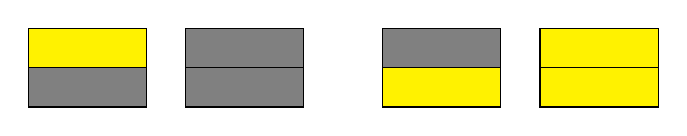
\begin{tikzpicture}[scale=0.5]
			\fill[gray] (0,0) rectangle (3,1);
			\fill[yellow] (0,1) rectangle (3,2);
			\fill[gray] (9,1) rectangle (12,2);
			\fill[yellow] (9,0) rectangle (12,1);
			\fill[gray] (4,0) rectangle (7,2);
			\fill[yellow] (13,0) rectangle (16,2);
			
			\foreach \i in {0,4,9,13}{
			\draw (\i,0) rectangle (\i+3,2);
			\draw (\i,1) -- (\i+3,1);}
		\end{tikzpicture}
		\caption{Todos los posibles arreglos de una pila, ninguno de estos es un arreglo justo.}
		\label{F(1)}
	\end{figure}
	
	Ahora bien, usando a \ref{F(1)}, podemos construir los siguientes arreglos:
	\begin{figure}[htb!]
		\centering
		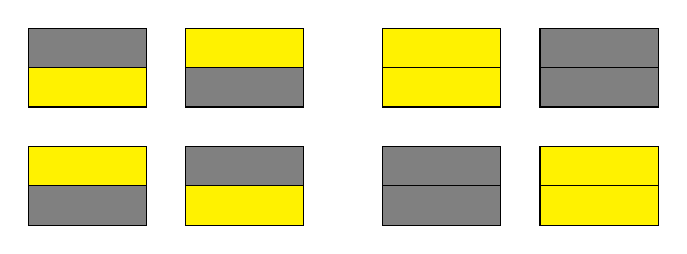
\begin{tikzpicture}[scale=0.5]
			\fill[gray] (0,0) rectangle (3,1);
			\fill[yellow] (0,1) rectangle (3,2);
			\fill[gray] (4,1) rectangle (7,2);
			\fill[yellow] (4,0) rectangle (7,1);
			\fill[gray] (9,0) rectangle (12,2);
			\fill[yellow] (13,0) rectangle (16,2);
			
			\fill[yellow] (0,3) rectangle (3,4);
			\fill[gray] (0,4) rectangle (3,5);
			\fill[yellow] (4,4) rectangle (7,5);
			\fill[gray] (4,3) rectangle (7,4);
			\fill[yellow] (9,3) rectangle (12,5);
			\fill[gray] (13,3) rectangle (16,5);
			
			
			
			\foreach \i in {0,4, 9, 13}{
				\draw (\i,0) rectangle (\i+3,2);
				\draw (\i,1) -- (\i+3,1);
				
				\draw (\i,3) rectangle (\i+3,5);
				\draw (\i,4) -- (\i+3,4);}
		\end{tikzpicture}
		\caption{Arreglos justos con \(F(2)\).}
	\end{figure}
	
	Ahora bien, notemos que podemos combinar estos arreglos justos con las formas de colocar una pila; pero el arreglo solo será justo si la pila agregada mantiene invariante la forma en que los turnos pueden ser jugados; es decir, agregar una pila no altera la paridad de los turnos necesarios para hacer que un jugador no tenga ninguna jugada disponible. Note que si tenemos más monedas de algún tipo, esto hace que ese jugador tenga más jugadas disponibles, mientras hace que el otro tenga menos jugadas disponibles. Notemos entonces que para que uno de los jugadores no tenga jugadas disponibles es necesario que no hayan del tipo de fichas con las que el jugador hace sus movimientos; ahora bien, como queremos que ambos jugadores puedan llevar a esta condición a su rival, tendremos que deben existir igual cantidad de monedas de cada tipo. Entonces tendremos que las formas para \(F(3)\) serán
	
	\begin{figure}[htb!]
		\centering
		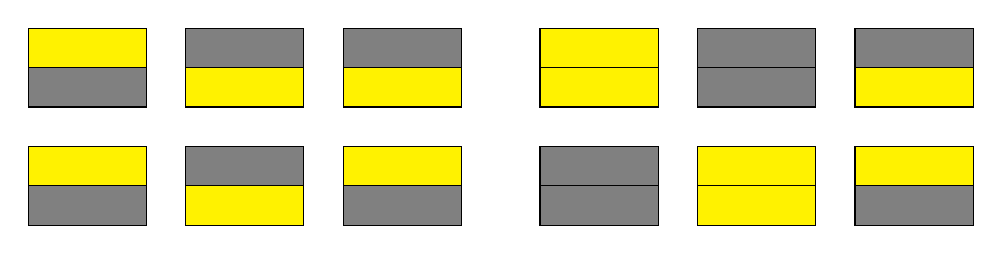
\begin{tikzpicture}[scale=0.5]
			\fill[gray] (0,0) rectangle (3,1);
			\fill[yellow] (0,1) rectangle (3,2);
			\fill[gray] (4,1) rectangle (7,2);
			\fill[yellow] (4,0) rectangle (7,1);
			\fill[gray] (8,0) rectangle (11,1);
			\fill[yellow] (8,1) rectangle (11,2);
			
			\fill[gray] (0,3) rectangle (3,4);
			\fill[yellow] (0,4) rectangle (3,5);
			\fill[gray] (4,4) rectangle (7,5);
			\fill[yellow] (4,3) rectangle (7,4);
			\fill[yellow] (8,3) rectangle (11,4);
			\fill[gray] (8,4) rectangle (11,5);
			
			\fill[gray] (13,0) rectangle (16, 2);
			\fill[yellow] (17,0) rectangle (20, 2);
			\fill[gray] (21,0) rectangle (24,1);
			\fill[yellow] (21,1) rectangle (24,2);
			
			
			\fill[yellow] (13,3) rectangle (16, 5);
			\fill[gray] (17,3) rectangle (20, 5);
			\fill[yellow] (21,3) rectangle (24,4);
			\fill[gray] (21,4) rectangle (24,5);
			
			\foreach \i in {0,4,8,13,17,21}{
				\draw (\i,0) rectangle (\i+3,2);
				\draw (\i,1) -- (\i+3,1);
				
				\draw (\i,3) rectangle (\i+3,5);
				\draw (\i,4) -- (\i+3,4);}
		\end{tikzpicture}
		\caption{En la figura tenemos las generadoras de todos los arreglos justos, note que los dos a la izquierda tienen \(3\) permutaciones, mientras que los dos a la derecha tiene \(6\) permutaciones cada uno, de esto \(F(3)=18\).}
		\label{F(3)}
	\end{figure}
	\newpage 
	
	Notemos que este proceso puede extender hacia cualquier \(n\), con la condición que, cuando \(n\) es par, entonces puede agregarse el caso donde tenemos \(\frac{n}{2}\) pilas todas con monedas de plata y la misma cantidad de pilas de monedas de oro. Es decir, se tiene que de las \(n\) pilas, esto genera \(2n\) monedas, se desea que \(n\) monedas sean de oro y \(n\) de plata; notemos además que en estas elecciones siempre se generan las distribuciones:
	
	\begin{figure}[htb!]
		\centering
		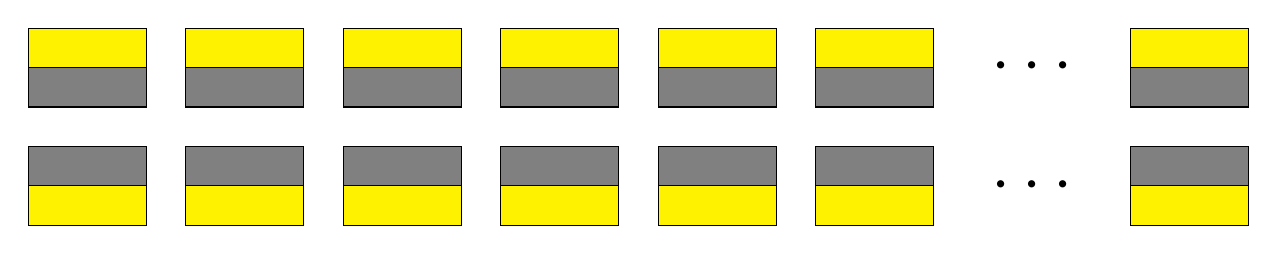
\begin{tikzpicture}[scale=0.5]
			\foreach \i in {0,4,...,20, 28}{
				\fill[yellow] (\i, 0) rectangle (\i+3,1);
				\fill[gray] (\i, 1) rectangle (\i+3,2);
				\fill[yellow] (\i, 4) rectangle (\i+3,5);
				\fill[gray] (\i, 3) rectangle (\i+3,4);}
			
			
			\foreach \i in {0,4,...,20, 28}{
				\draw (\i,0) rectangle (\i+3,2);
				\draw (\i,1) -- (\i+3,1);
				
				\draw (\i,3) rectangle (\i+3,5);
				\draw (\i,4) -- (\i+3,4);}
			\node () at (25.5, 1) {\Huge $\cdots$};
			\node () at (25.5, 4) {\Huge $\cdots$};
		\end{tikzpicture}
		\caption{Distribuciones no justas.}
		\label{nojust}
	\end{figure}
	
	Ahora bien, notemos que por cada pila de monedas de un solo tipo hay otra pila de monedas del otro  tipo. Mientras que si llamamos a la secuencia \(OP\) ser una pila de dos monedas con la moneda superior de oro y la inferior de plata, mientras que la secuencia \(PO\) es una pila de dos monedas con la superior de plata y la inferior de oro. Dado que siempre elegimos \(2n\) monedas, estas pueden ser de cuatro tipos, una pila de monedas de oro \((OO)\), una pila de monedas de plata \((PP)\), una pila \(OP\) o una fila \(PO\); resaltando que cada pila \(OO\) implica que hay una pila \(PP\), es decir, elegir una fila del tipo \(OO\) o del  tipo
	\(PP\) implica que se están eligiendo dos pilas, una de tipo \(OO\) y la otra de tipo \(PP\). Además de la gráfica \ref{nojust}, sabemos que si elegimos algún tipo de pila, entonces esta no puede ser el único tipo de pila que utilicemos, es decir, debemos elegir al menos dos tipos de pila distintos, aunque los elijamos de manera desigual, es decir, un arreglo justo puede consistir de \(n-1\) pilas del tipo \(OP\) y una pila \(PO\).
	
	De esto, notamos una estructura bastante interesante, todos los arreglos justos para \(n\) pilas pueden contarse de la forma:
	\begin{align*}
		F(n) &:= \binom{n}{0,0, n-1, 1} + \binom{n}{0,0, n-2, 2} + ... + \binom{n}{0,0, 1, n-1} + \binom{n}{1,1, n-2, 0} + \binom{n}{1,1, n-3, 1} + \\
		&=... + \binom{n}{1,1, 0, n-2} + ... + \binom{n}{\floor{\frac{n}{2}},\floor{\frac{n}{2}}, n-2\floor{\frac{n}{2}}, 0}\\
		&= \left(\sum_{i=0}^{\floor{\frac{n}{2}}} \sum_{j=0}^{n-i} \binom{n}{i, i, j, (n-2i-j)} \right)-2
	\end{align*}
	
	por ello se implementa la función mostrada en el código.
	
	
	\section{Problema 2}
	
	Notemos que para saber si un número es abundante o no, solo es necesario saber si la suma de sus divisores propios es o no mayor que el número, entonces necesitamos calcular sus divisores propios, esto es sencillo, pues solo necesitamos el bucle \texttt{for} que generamos al inicio de nuestro código, dentro de la definición de nuestra función \texttt{esAbundante}, ya que hemos calculado todos sus divisores propios, tendremos que  sumarlos y esto se resuelve con otro bucle \texttt{for} a través de la lista \texttt{a} que definimos en la función; una vez suma, solo nos falta verificar si la suma de divisores propios es mayor que el número, para ello condicionamos el retorno de nuestra función, para que si se cumple la condición, se tenga devuelva \textcolor{blue}{\texttt{True}} y en cualquier otro caso se devuelva \textcolor{blue}{\texttt{False}}.
	
	Ahora bien, notemos que con esto, ya solo verificamos en el rango desde el \(12\) hasta \(28123\), con esto obtenemos todos los números abundantes en ese rango; guardándolos en la lista \texttt{listaAbun}, luego verificamos si cada uno de los números en el rango de \(1\) a \(28123\) si pueden escribirse como suma de dos números abundantes, los guardamos en la lista \texttt{lista2Abun}.
	
	Ya que tenemos la lista anterior, procedemos a verificar si los números entre el \(24\) y el \(28123\) son suma de dos abundantes, en caso eso no ocurra, los guardaremos en la lista \texttt{listaNoAbun}. Luego iniciamos una variable para guarda la suma llamada \texttt{noAbunSum}, para luego usar un \texttt{for} y agregarle cada valor de la lista de los que no se puede escribir como suma de dos abundantes.
	
	Luego imprimimos el valor obtenido y el tiempo que tomó encontrarlo. Obteniendo que la suma de todos los números no abundantes es \(297557279\). La ejecución del programa no toma más de \(10\) segundos.
	
	\section{Problema 3}
	
	Dado que queremos formar un rectángulo, solo basta con que hayan \(2\) parejas disjuntas de números que sean iguales, es decir necesitamos que \(a=b, c=d\) o \(a=c, b=d\) ó \(a=d, b=c\); entonces solo es necesario formar \(3\) casos de evaluación. Para ello, formamos la estructura que nos pide el problema dando un entero \(T\) como inicio, formamos un bucle \texttt{for} de duración \(T\) y al inicio de cada ciclo guardamos y separamos los \(4\) enteros que son los lados; así mismo asignamos los cuatro enteros en una línea mediante comas y procedemos a comparar los casos anteriores en donde verificamos la primera parte y luego la segunda, si se cumplen ambas imprimimos \texttt{YES} y si no se cumplen ninguna de las tres condiciones iniciales imprimimos \texttt{NO}.
	
	\section{Enlaces a los códigos de Python}
	
	\subsection{Problema 1}
	
	El código se encuentra en el siguiente \href{URL}{link}.
	
	\subsection{Problema 2}
	
	El código se encuentra en el siguiente \href{URL}{link}.
	
	\subsection{Problema 3}
	
	El código se encuentra en el siguiente \href{URL}{link}.
	
\end{document}